\documentclass[uplatex,dvipdfmx]{jsarticle}

\usepackage[uplatex,deluxe]{otf} 
\usepackage[noalphabet]{pxchfon} 
\usepackage{stix2} 
\usepackage[fleqn,tbtags]{mathtools} 
\usepackage{amsmath}
\usepackage{url}
\usepackage{float}
\usepackage{xurl}
\usepackage{graphicx}
\usepackage{array}
\usepackage{tabularx}

% --- ここから追加 ---
\usepackage{tikz}
\usetikzlibrary{arrows.meta, positioning, shapes.geometric}
% --------------------
\begin{document}

\title{\textbf{Arduino演奏システム設計書}}
\author{25G1051 近藤巧望}
\date{\today}
\maketitle

\section{\textbf{システムの基本設計}}

\subsection{\textbf{機能一覧}}

トロンボーンユニットの主要機能とその詳細を表\ref{tab:functions}にまとめる．
実装にあたっては，これらの機能が相互に連携し，リアルタイムな演奏制御を実現することが求められる．

Processingにおいて，トロンボーンの音色は振幅で制御するためF2.1の振幅ベース音色制御が重要な役割を果たす．
音響物理学・音色合成に関する理論では，加算合成法に基づき，基本周波数とその倍音成分の振幅比率を調整することで特定の楽器音色を模倣できることが知られている\cite{AdditiveSynthesis}．

\begin{table}[H]
\centering
\renewcommand{\arraystretch}{1.3} % 行間に少し余裕を持たせる
\small
\begin{tabularx}{\textwidth}{|l|>{\raggedright\arraybackslash}X|>{\raggedright\arraybackslash}X|>{\raggedright\arraybackslash}X|}
\hline
 \textbf{ID} & \textbf{主要機能} & \textbf{機能詳細・役割} & \textbf{対応要素} \\ \hline
 \textbf{F1.0} & \textbf{データ同期制御} & 外部入力値を内部演奏パラメータへ動的にマッピングする． & - \\ \hline
 F1.1 & パラメータ同期受信 & ArduinoからのBPM・音名データを変数へ即時反映し同期させる． & \texttt{currentBpm}, \texttt{currentNote} \\ \hline
 F1.2 & 演奏時間動的計算 & 受信したBPM値に基づき，音価に対応した実時間を算出する． & \texttt{beatLength}, \texttt{noteLength} \\ \hline
 \textbf{F2.0} & \textbf{音響信号生成系} & パラメータ制御による波形合成および信号処理を行う． & - \\ \hline
 F2.1 & 振幅ベース音色制御 & 各倍音の振幅値（比率）を直接指定し，トロンボーン音色を合成する． & \texttt{wave1 \~{} wave4}, \texttt{amp} \\ \hline
 F2.2 & 音階・周波数変換 & 受信した音名文字列を，DSP処理用の周波数データへ変換する． & \texttt{noteToFreq()} \\ \hline
 F2.3 & 信号エンベロープ処理 & 指定された振幅最大値（maxAmp）に基づき，時間的減衰を制御する． & \texttt{Line (env1 \~{} env4)} \\ \hline
 \textbf{F3.0} & \textbf{出力・表示} & 処理結果を視聴覚情報としてユーザへ提示する． & - \\ \hline
 F3.1 & 内部状態表示 & BPM，Note名，振幅設定値などの稼働パラメータを文字表示する． & \texttt{draw()} \\ \hline
\end{tabularx}
\caption{トロンボーンシステム機能一覧表}
\label{tab:functions}
\end{table}

\subsection{\textbf{システム構成図}}
トロンボーンユニットのシステム構成を図\ref{fig:system_kousei}に示す．
UI/制御系はPC上のブラウザで実装され，ArduinoサーバーとWiFi（HTTP/OSC）を介して通信する．
Arduinoサーバーは，受信したBPM情報をもとに全体の演奏テンポを管理し，トロンボーンユニットを含む各楽器ユニットへ同期信号（パルス信号）を小節ごとに送信する．
トロンボーンユニットは，受信した同期信号に基づいて自身の演奏タイミングを確定させ，Processingへ演奏開始のトリガーを送信する．
Processingは，受信したトリガーに基づいて音響信号（振幅制御による合成音声）を生成し，PC内蔵スピーカーから出力する．

\begin{center}
\begin{figure}[H]
        
\includegraphics[width=1.0\textwidth]{system.png}
        \caption{トロンボーン部分のシステム構成図．
        表\ref{tab:functions}の機能IDを対応させて記載している．}
        \label{fig:system_kousei}
\end{figure}
\end{center}

\subsection{\textbf{操作インターフェース設計}}
ユーザは，PC上のブラウザに実装されたWeb UIを通じてシステムを操作する．本インターフェースは以下の機能を備える．
\begin{itemize}
    \item \textbf{BPM入力フィールド：} 楽曲のテンポを指定し，ArduinoサーバーへWiFi（HTTP/OSC）経由で送信する．
    \item \textbf{接続ステータス表示：} 各Arduinoユニットとの通信確立状況をリアルタイムで確認できる．
    \item \textbf{演奏制御ボタン：} シーケンスの開始（送信）および強制停止を命令する．
\end{itemize}

\subsection{\textbf{状態遷移図}}
本ユニット（Arduino トロンボーン）は，外部機器との同期を自動的に行うため，図\ref{joutai}に示す4つの状態を遷移する．各状態は機能一覧の各項目と密接に関連している．

\begin{figure}[H]
    \centering
    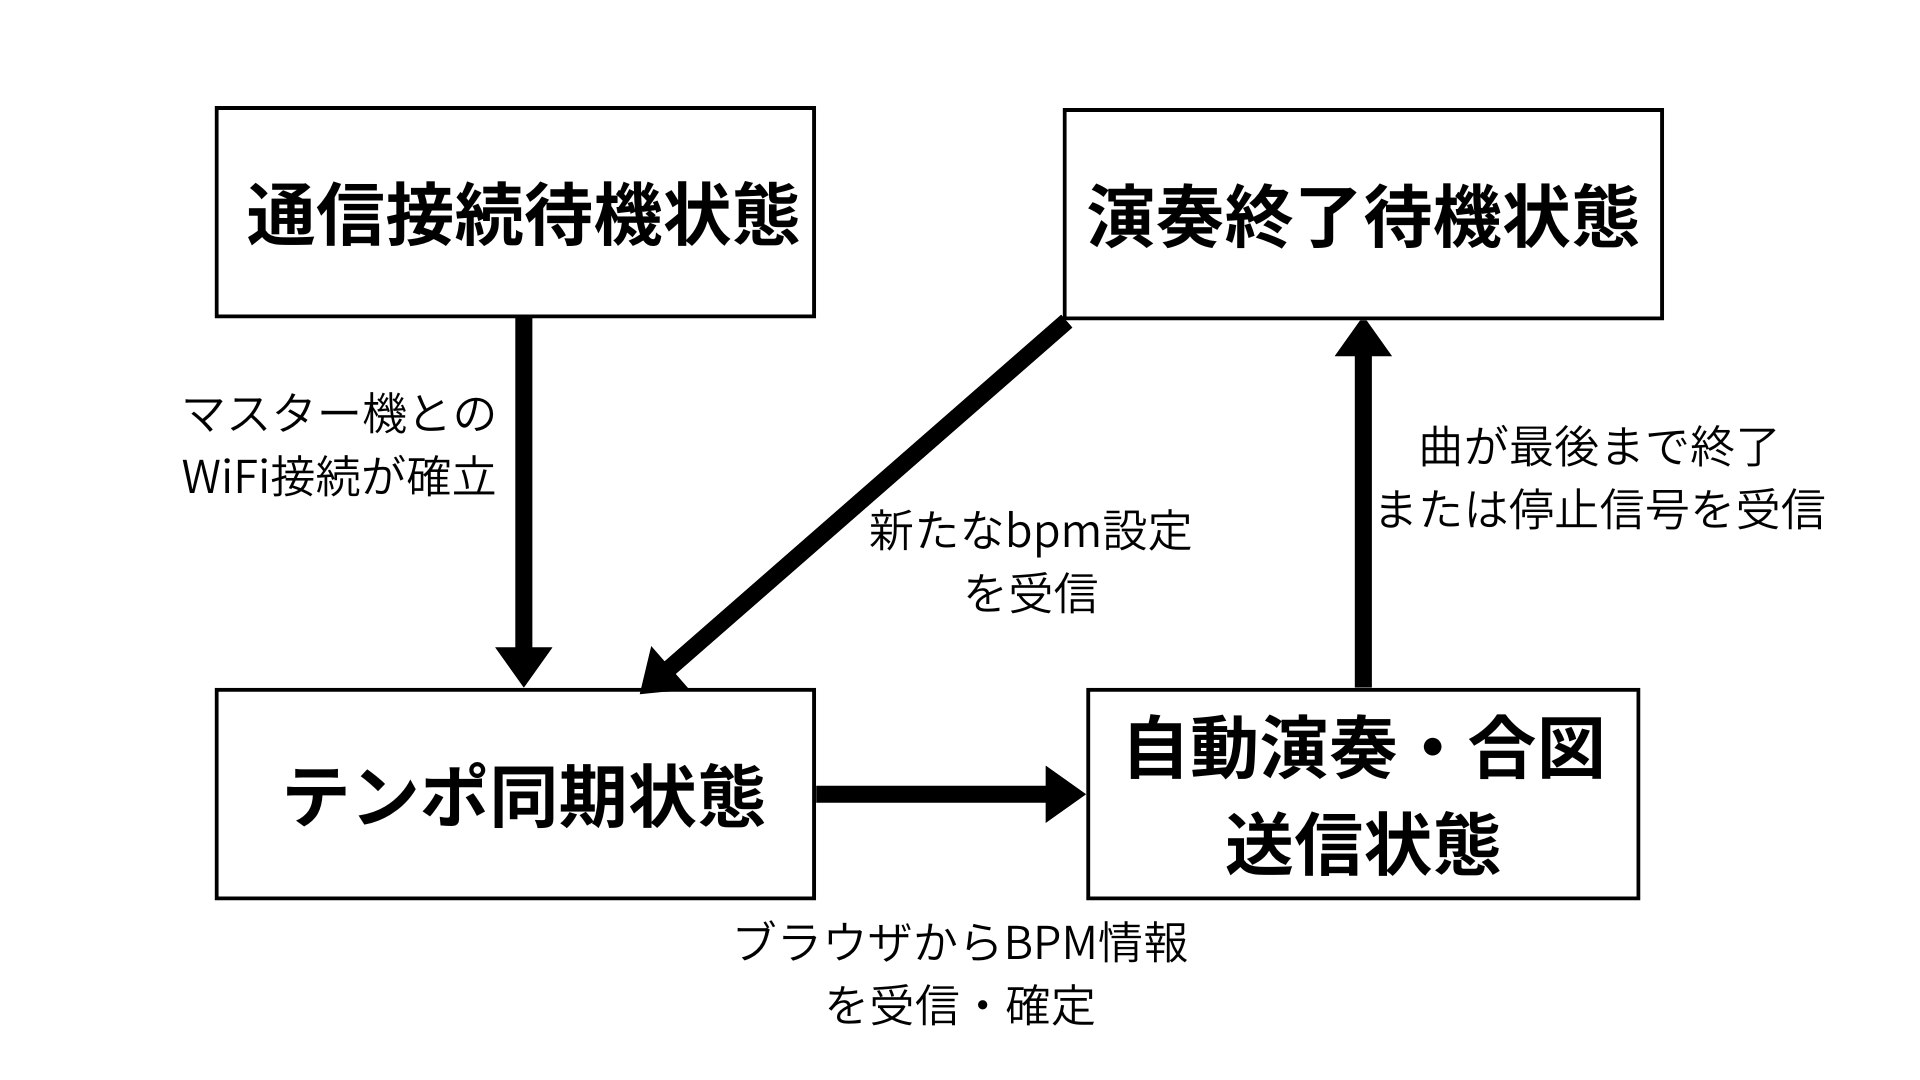
\includegraphics[width=0.9\textwidth]{joutai.png}
    \caption{トロンボーンユニットの状態遷移図}
    \label{joutai}
\end{figure}

各状態の役割および遷移条件の詳細を以下に示す．

\begin{itemize}
\item \textbf{1．通信接続待機状態：}
電源投入後の初期状態である．Arduino サーバーとのWiFi接続を確立し，データの受信準備を整える．接続の確立が次状態へのトリガーとなる．
\item \textbf{2．テンポ同期状態（F1.1，F1.2）：}
ブラウザUIから確定されたBPM情報を受信し，内部変数（\texttt{currentBpm}）を更新する状態である．受信した数値に基づき，音価（音符の長さ）に対応する実時間を計算する．
\item \textbf{3．自動演奏・合図送信状態（F2.0全般）：}
演奏開始信号を受信した瞬間に移行する実行状態である．プログラムされた音階データを処理しつつ，第1拍目のタイミングでProcessingへ同期トリガーを送信する．この間，振幅制御に基づいた音声合成が並行して実行される．
\item \textbf{4．演奏終了待機状態：}
楽曲の終了，または手動の停止信号を受信した際の安全状態である．すべての音声出力を停止し，変数をリセットする．新たなBPM設定を受信することで，再び「テンポ同期状態」へと復帰する．
\end{itemize}

\section{\textbf{システムの詳細設計}}

\subsection{\textbf{部品・ソフトウェア一覧}}
本システムの構築に使用するハードウェアおよびソフトウェア一式を表\ref{tab:parts}に示す．
\indent
まず，前提としてOSはmacOSを使用する．
また，Arduino Uno R4はWiFi通信機能を内蔵しているため，外部モジュールは必要ない．
スピーカーに関してはPC内蔵のものを使用するため，特別なオーディオインターフェースも不要である．
音声を作成するためのProcessingでは，Minimライブラリを使用する．
MinimはProcessingで⾳響処理をするためのライブラリであり，波形の合成やエンベロープ制御などの機能を提供する\cite{Minim}．
更に，Arduinoにプログラム書き込むためにはArduino IDEを使用する．
通信プロトコルは，UDPをベースとしたOSC（Open Sound Control）を採用する．OSCは音楽やマルチメディアアプリケーション間の通信に特化したプロトコルであり，低遅延かつ柔軟なデータ構造を持つため，本システムのリアルタイムな演奏同期に適している\cite{OSC}．

\begin{table}[H]
\centering
\renewcommand{\arraystretch}{1.2}
\small
\begin{tabularx}{\textwidth}{|l|>{\raggedright\arraybackslash}X|>{\raggedright\arraybackslash}X|}
\hline
 \textbf{分類} & \textbf{名称・型番} & \textbf{用途・備考} \\ \hline
 \textbf{ハードウェア} & PC & Processingの実行，ブラウザUIのホスト． \\ \cline{2-3}
  & Arduino Uno R4 WiFi & サーバー機およびトロンボーン機として計2台使用(他楽器を含めると全部で5台使用)．WiFi通信機能必須． \\ \cline{2-3}
 \textbf{ソフトウェア} & Processing & 音響合成エンジンおよびメインシーケンサー． \\ \cline{2-3}
  & Minim ライブラリ & Processing上での波形合成，エンベロープ制御． \\ \cline{2-3}
  & Arduino IDE & マイコン用制御プログラムの開発． \\ \cline{2-3}
 \textbf{通信プロトコル} & UDP / OSC (Open Sound Control) & 各ユニット間での低遅延な演奏同期信号の送受信． \\ \hline
\end{tabularx}
\caption{部品・ソフトウェア一覧}
\label{tab:parts}
\end{table}

\subsection{\textbf{ハードウェア設計}}
本項では，前節の表\ref{tab:parts}に基づき，トロンボーンユニットの具体的な接続関係および動作仕様について述べる．

\subsubsection{周辺部品の詳細仕様}
本ユニットは，サーバーから受信する小節番号および同期信号に基づき，あらかじめプログラムされたシーケンスを自動実行する構成をとる．
そのため，物理入力はシステム全体のテンポ調整に特化しており，タクトスイッチを用いてBPMの増減を行う．

\begin{table}[H]
\centering
\caption{使用部品の詳細仕様}
\label{tab:hardware_spec_final}
\renewcommand{\arraystretch}{1.2}
\small
\begin{tabularx}{\textwidth}{|l|l|l|X|}
\hline
\textbf{名称} & \textbf{型番・メーカー} & \textbf{端子/ピン} & \textbf{特性・役割} \\ \hline
BPM変更ボタン & タクトスイッチ (12mm角) & D2 & 演奏テンポ（BPM）を段階的に切り替えるための物理入力． \\ \hline
給電用ケーブル & USB Type-C ケーブル & 電源入力 & Arduino Uno R4 WiFiへの給電およびプログラム書き込み用． \\ \hline
\end{tabularx}
\end{table}

\subsubsection{回路構成と接続インターフェース}
Arduino Uno R4 WiFiを中心とした接続構成を図\ref{fig:kairo}に示す．

%\begin{figure}[H]
%    \centering
%    \includegraphics[width=0.7\textwidth]{kairo.png} 
%    \caption{トロンボーンユニット回路構成図（BPM制御部）}
%    \label{fig:kairo}
%\end{figure}

具体的な回路接続としては，タクトスイッチの一方を \texttt{D2} ピン，もう一方をGNDに接続する．
Arduino内部のプルアップ抵抗（\texttt{INPUT\_PULLUP}）を有効化し，押下時に \texttt{LOW} となるアクティブロー構成を採用する．

\subsubsection{ハードウェア動作の具体化}
各部品および通信機能が連携し，演奏同期を実現するプロセスを以下に定義する．

\begin{enumerate}
    \item \textbf{ネットワーク同期による自動演奏開始：} 
    本ユニットは，ArduinoサーバーからWiFi（UDP/OSC）経由で配信される「小節番号パケット」を常時監視する．自身の担当する小節番号を受信した瞬間に演奏フラグを立て，Processingへ音響生成のトリガーを送出する．
    \item \textbf{物理ボタンによるBPM同期：} 
    \texttt{D2} ピンの入力を検知した際，プログラム内のBPM変数を更新し，その変更をOSCパケットとして他ユニット（サーバー等）へ即座に共有する．
    \item \textbf{通信モジュールの最適化：} 
    Arduino Uno R4 WiFiの内蔵モジュールを用いることで，外部配線によるノイズや断線リスクを排除し，パケット受信から処理開始までの遅延（レイテンシ）を最小化している．
\end{enumerate}
\subsection{\textbf{ソフトウェア設計}}

\subsubsection{\textbf{ファイル構成}}
\begin{itemize}
\item \texttt{Main.ino}：メインループおよびシステム全体の動作状態管理．
\item \texttt{OscParser.cpp / .h}：受信したWeb OSCメッセージ（BPM，開始合図）の解析．
\item \texttt{AudioEngine.cpp / .h}：BPMに同期したタイマー管理および音響生成ロジック．
\item \texttt{NetworkConfig.h}：WiFi接続情報および外部同期先のIPアドレス定義．
\end{itemize}

\subsubsection{\textbf{オブジェクト設計（クラス図）}}
\begin{itemize}
\item \textbf{BpmReceiverクラス：} ブラウザから送信されたBPM値を取得し，システム変数へ反映する．
\item \textbf{PlayManagerクラス：} 自動演奏のタイミング制御およびメロディデータの読み出しを行う．
\item \textbf{SyncSenderクラス：} 演奏開始と同時にProcessing宛てのOSCパケットを構築・送出する．
\end{itemize}

\subsubsection{\textbf{関数設計}}
\begin{itemize}
\item \texttt{void receiveBpm()}：UDPポートを監視し，BPM値が含まれるパケットを受信した際に内部数値を更新する．
\item \texttt{void updateTimerInterval(float bpm)}：BPMをタイマー割り込み周期へ変換し，ハードウェアレジスタへ即座に反映する．
\item \texttt{void broadcastTrigger()}：演奏の第1拍目に合わせ，無線ネットワーク経由で開始合図を射出する．
\end{itemize}

\subsection{\textbf{処理フローの設計}}
本システムは，以下の3段階の自動化フローによって動作する．
\begin{enumerate}
\item \textbf{初期化：} 起動時にWiFi接続を確立し，外部からのOSCパケット受信を待機する．
\item \textbf{同期：} ブラウザUIでの操作（BPM確定）を受け，内部の演奏タイマーをマスター機と同期させる．
\item \textbf{実行：} 確定したテンポで自動演奏を開始し，同時にProcessingへ向けて「演奏開始合図」を自動送信する．
\end{enumerate}

また，図\ref{flow}に処理フローの概要を示す．
\begin{center}
\begin{figure}[H]
        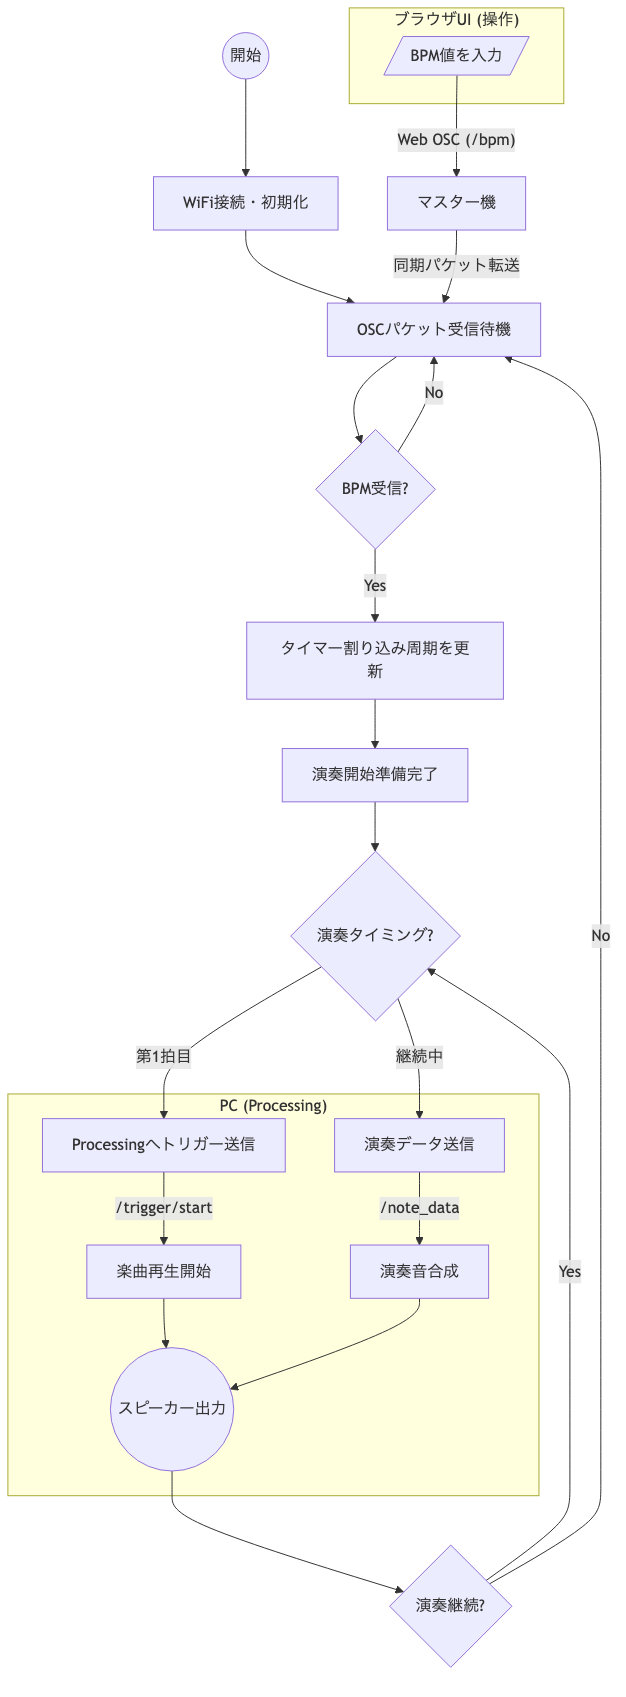
\includegraphics[width=0.5\textwidth]{flow.png}
        \caption{トロンボーン部分の処理フロー図}
        \label{flow}
\end{figure}
\end{center}

\subsection{\textbf{テストの設計}}
\begin{itemize}
\item \textbf{データ整合性テスト：} ブラウザ上で入力したBPM値が，トロンボーン側で正確な演奏周期として反映されているかを確認する．
\item \textbf{同時再生テスト：} トロンボーンの第1拍目の発音と，Processing側の伴奏再生の開始が完全に一致するかを確認する．
\item \textbf{非接触制御テスト：} 物理的な接点を一切持たず，ネットワーク経由のデータ通信のみで一連の動作が完結することを確認する．
\end{itemize}

\begin{thebibliography}{99}
        \bibitem{AdditiveSynthesis} N. H. Fletcher and T. D. Rossing (2012). The physics of musical instruments. \url{https://books.google.com/books?hl=ja&lr=lang_ja/lang_en&id=gvDSBwAAQBAJ&oi=fnd&pg=PR5&dq=N.+H.+Fletcher+%26+T.+D.+Rossing+%22The+Physics+of+Musical+Instruments%22&ots=noY7enAyw9&sig=StlTtAdA4Qiw9_d_x1au4-K37Mw}
        \bibitem{Minim} Minim document. \url{https://code.compartmental.net/minim/}
        %以下，まだ調べていない参考文献
        \bibitem{OSC} Wright, M., \& Freed, A. (1997). Open Sound Control: A New Protocol for Communicating with Sound Synthesizers. Proceedings of the International Computer Music.\url{https://www.adrianfreed.com/sites/default/files/open-soundcontrol-a-new-protocol-for-communicating-with.pdf}
\end{thebibliography}

\end{document}